\section{Dataset} \label{dataset}
This paper builds on data captured by TTNet \cite{voeikov2020ttnet} and released by OSAI \cite{OSAI}. The data includes match and player statistics from Tischtennis-Bundesliga, the top professional German table tennis league, as well as men and women's singles matches from the Tokyo 2020 Olympics. Many potential features such as player age, rank, match duration as well as in-match statistics such as percentage of points won on serve and receive, stroke types and error types are available. Interactive maps that demonstrated the ball position of each shot on the table, as well as the stroke type were also accessible. The progression of a rally and location of each ball bounce can be mapped into a sequence (e.g. see Figure \ref{sequence}).

%\denes{Can we say that one of the challenges is to find out which features might be salient for a result predictor?}

\begin{figure}[ht]
\centering

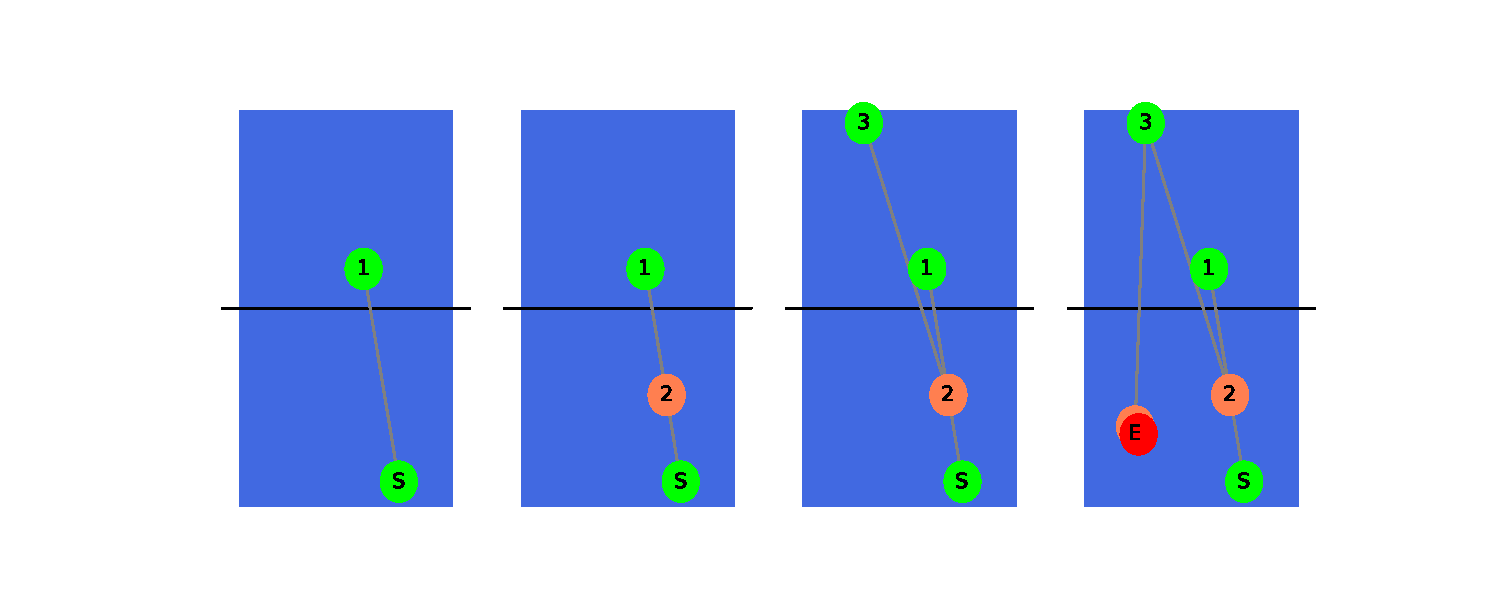
\includegraphics[width=8.5cm]{plots/tablesequence.pdf}
\caption{Progression of a rally demonstrating the landing point of each ball bounce. Yellow indicates service which starts a rally and red indicates an error ending the rally. Green indicates all other ball bounces \cite{OSAI}.}

\label{sequence}
\end{figure}

From this, each half of the table can be split into nine equal sections, and the location of every winning shot of the match can be grouped into one of these parts, as shown in Figure \ref{pos}.

\begin{figure}[ht]
\centering

%\vspace{-2em}
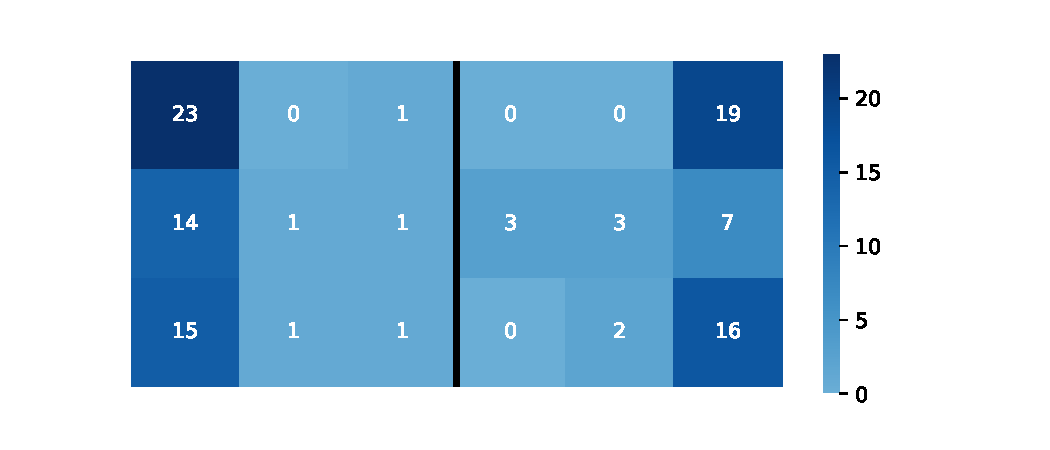
\includegraphics[width=8cm]{plots/tableheatmaprot.pdf}
\caption{Distribution of ball placement of a winning shot for both players by region if each side of the table were to be split into nine equal parts. Each value indicates the number of balls landing in it's respective region \cite{OSAI}.}

\label{pos}
\end{figure}

The number of forehands and the number of backhands used to win a point can be accumulated and grouped. Similarly, the number of rallies can be totalled by the location of the last bounce, and whether it was 'short` or 'long`. For examples, refer to Figures \ref{fvbh} and \ref{svlr}. We will use this data to measure the strength of different skills of a player in different aspects of the sport.

\begin{figure}[ht]
\centering

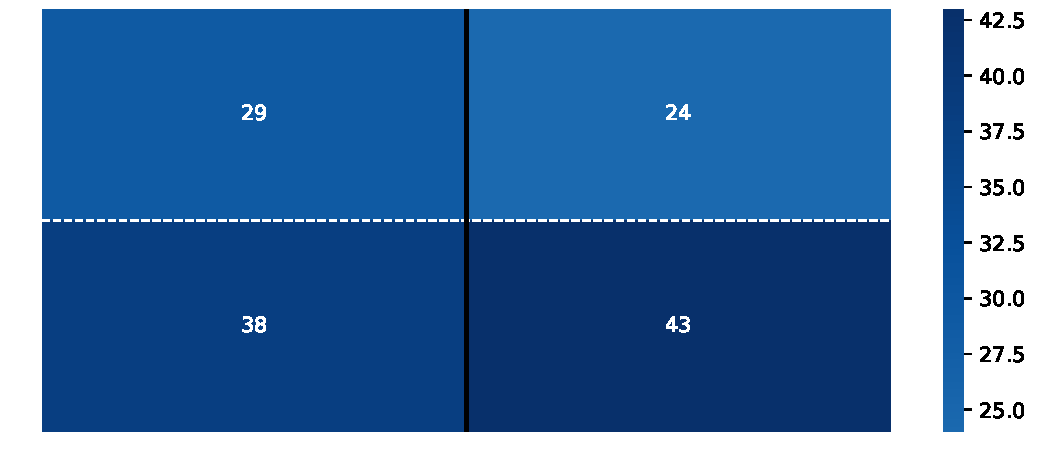
\includegraphics[width=8cm]{plots/forehandvsbackhand.pdf}
\caption{Distribution of points won by forehand compared to a backhand \cite{OSAI}.}

\label{fvbh}
\end{figure}

\begin{figure}[ht]
\centering

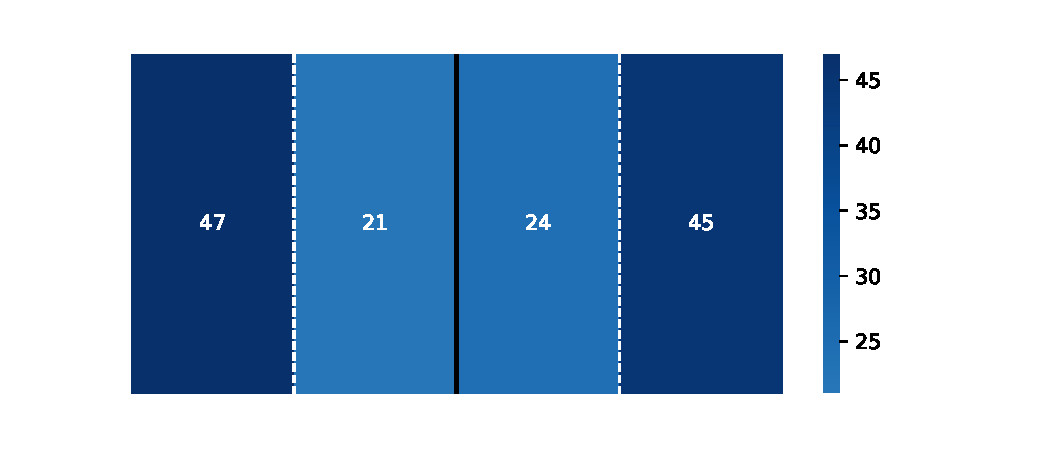
\includegraphics[width=8cm]{plots/shortvslongrally.pdf}
\caption{Distribution of points won by a short rather than long rally \cite{OSAI}.}

\label{svlr}
\end{figure}


 Samples with missing data entries were removed from the dataset. One of the main challenges in constructing a successful result predictor is the selection of salient features. To address this, we carefully hand picked features that we thought would be the most influential in a match based on existing domain knowledge on the problem.